%%%%%%%%%%%%%%%%%%%%%%%%%%%%%%%%%%%%%%%%%%%%%%%%%%%%%%%%%%%%%%%%%%%%%%%%%%%%%%%%%%%%%%%%%%%%%%%%%%%%%%%%%%%%%%%%%%%%%%%%%%%%%%%%%%%%%%%%%%%%%%%%%%%%%%%%%%%%%%%%%%%
% Written By Michael Brodskiy
% Class: Analysis of Random Phenomena
% Professor: I. Salama
%%%%%%%%%%%%%%%%%%%%%%%%%%%%%%%%%%%%%%%%%%%%%%%%%%%%%%%%%%%%%%%%%%%%%%%%%%%%%%%%%%%%%%%%%%%%%%%%%%%%%%%%%%%%%%%%%%%%%%%%%%%%%%%%%%%%%%%%%%%%%%%%%%%%%%%%%%%%%%%%%%%

\documentclass[12pt]{article} 
\usepackage{alphalph}
\usepackage[utf8]{inputenc}
\usepackage[russian,english]{babel}
\usepackage{titling}
\usepackage{float}
\usepackage{amsmath}
\usepackage{graphicx}
\usepackage{enumitem}
\usepackage{amssymb}
\usepackage[super]{nth}
\usepackage{everysel}
\usepackage{ragged2e}
\usepackage{geometry}
\usepackage{multicol}
\usepackage{fancyhdr}
\usepackage{cancel}
\usepackage{siunitx}
\usepackage{physics}
\usepackage{tikz}
\usepackage{mathdots}
\usepackage{yhmath}
\usepackage{cancel}
\usepackage{color}
\usepackage{xcolor}
\usepackage{colortbl}
\usepackage{array}
\usepackage{multirow}
\usepackage{gensymb}
\usepackage{tabularx}
\usepackage{extarrows}
\usepackage{booktabs}
\usepackage{lastpage}
\usetikzlibrary{fadings}
\usetikzlibrary{patterns}
\usetikzlibrary{shadows.blur}
\usetikzlibrary{shapes}

\geometry{top=1.0in,bottom=1.0in,left=1.0in,right=1.0in}
\newcommand{\subtitle}[1]{%
  \posttitle{%
    \par\end{center}
    \begin{center}\large#1\end{center}
    \vskip0.5em}%

}
\usepackage{hyperref}
\hypersetup{
colorlinks=true,
linkcolor=blue,
filecolor=magenta,      
urlcolor=blue,
citecolor=blue,
}


\title{Homework 10}
\date{\today}
\author{Michael Brodskiy\\ \small Professor: I. Salama}

\begin{document}

\maketitle

\begin{enumerate}

  \item We begin by writing an expression for $B_k=0$, which gives us a waveform of:

    $$x_0(t)=\cos\left( \frac{2\pi N t}{T} \right),\quad t\in[(k-1)T,kT]$$

    We then write, for $B_k=1$:

    $$x_0(t)=-\sin\left( \frac{2\pi N t}{T} \right),\quad t\in[(k-1)T,kT]$$

    We know that, given that $f_o$ is a multiple of $1/T$, we know a full $N$ cycles will be transmitted. We may observe that the sample space of $X$ consists of $8$ waveforms, as a result of the transmission of 3 bits (which means $2^3$ possible combinations. These are given by:

      $$x_o(t),\quad t\in[0,3T]$$
      $$x_o(t),\quad t\in[0,2T]\quad\text{ and }\quad x_1(t),\quad t\in[2T,3T]$$
      $$x_o(t),\quad t\in[0,T]\cup[2T,3T]\quad\text{ and }\quad x_1(t),\quad t\in[T,2T]$$
      $$x_o(t),\quad t\in[T,3T]\quad\text{ and }\quad x_1(t),\quad t\in[0,T]$$
      $$x_o(t),\quad t\in[0,T]\quad\text{ and }\quad x_1(t),\quad t\in[T,3T]$$
      $$x_o(t),\quad t\in[T,2T]\quad\text{ and }\quad x_1(t),\quad t\in[0,T]\cup[2T,3T]$$
      $$x_o(t),\quad t\in[2T,3T]\quad\text{ and }\quad x_1(t),\quad t\in[0,2T]$$
      $$x_1(t),\quad t\in[0,3T]$$

      Accordingly, we find that the elements correspond to $(B_1,B_2,B-3)$ as:

      $$X_k(t)\to\left\{\begin{array}{ll} 1, & (0,0,0)\\ 2, & (0,0,1)\\3, & (0,1,0)\\4, & (1,0,0)\\5, & (0,1,1)\\6, & (1,0,1)\\7, & (1,1,0)\\8, & (1,1,1)\\\end{array}$$

        To plot, we need to assume a value of $N$. Let us take this such that $N=T$ to simplify the functions. We proceed to plot each corresponding figure:

        \begin{figure}[H]
          \centering
          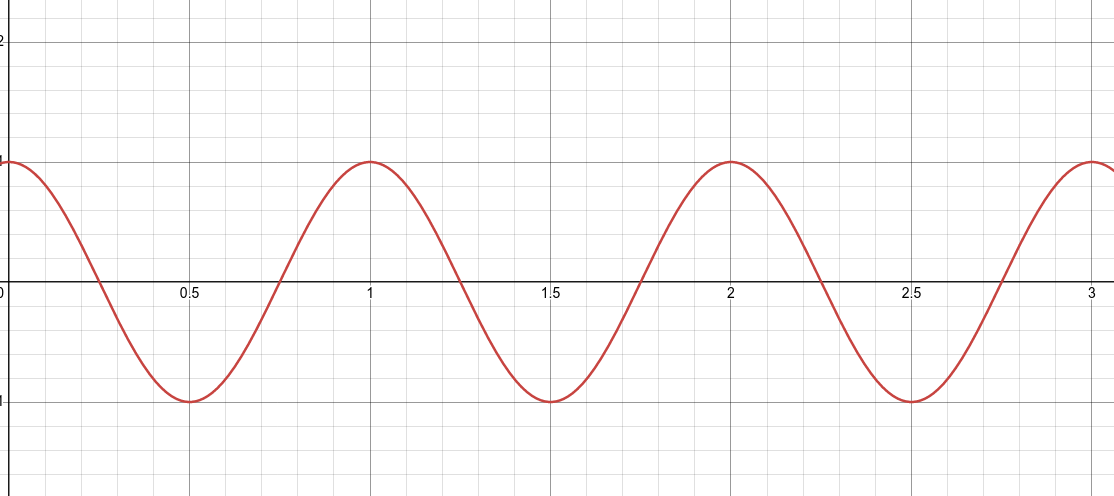
\includegraphics[width=.75\textwidth]{Figures/HW10-1a}
          \caption{Plot for $(B_1,B_2,B_3)=(0,0,0)$}
          \label{fig:1}
        \end{figure}

        \begin{figure}[H]
          \centering
          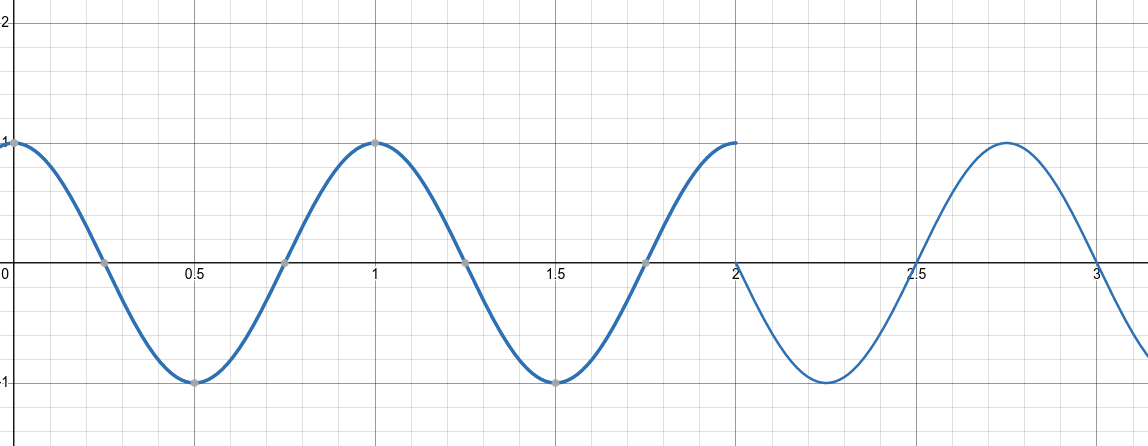
\includegraphics[width=.75\textwidth]{Figures/HW10-1b}
          \caption{Plot for $(B_1,B_2,B_3)=(0,0,1)$}
          \label{fig:2}
        \end{figure}

        \begin{figure}[H]
          \centering
          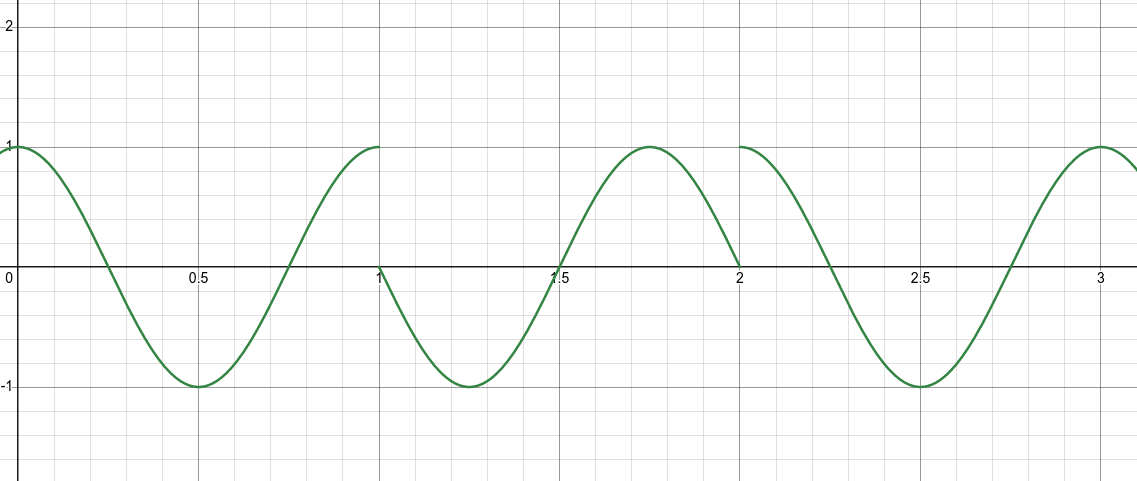
\includegraphics[width=.75\textwidth]{Figures/HW10-1c}
          \caption{Plot for $(B_1,B_2,B_3)=(0,1,0)$}
          \label{fig:3}
        \end{figure}

        \begin{figure}[H]
          \centering
          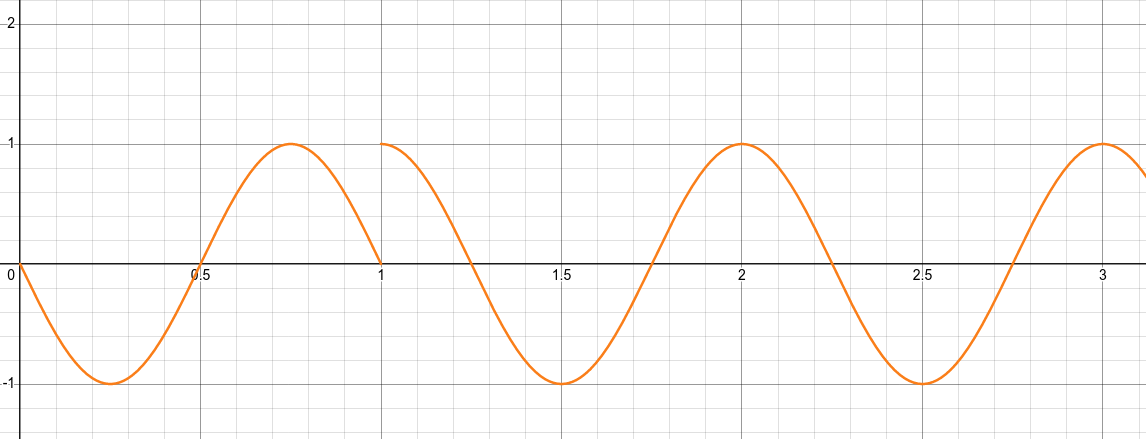
\includegraphics[width=.75\textwidth]{Figures/HW10-1d}
          \caption{Plot for $(B_1,B_2,B_3)=(1,0,0)$}
          \label{fig:4}
        \end{figure}

        \begin{figure}[H]
          \centering
          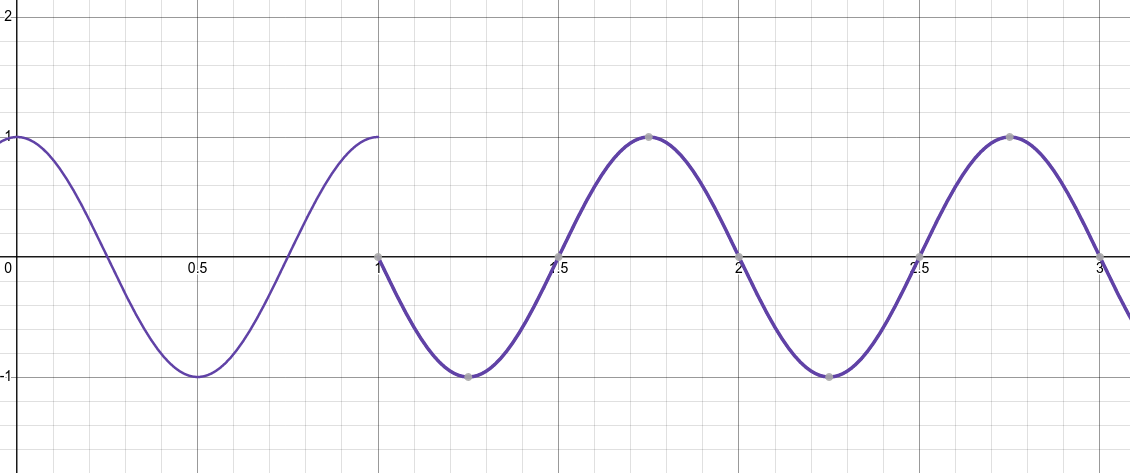
\includegraphics[width=.75\textwidth]{Figures/HW10-1e}
          \caption{Plot for $(B_1,B_2,B_3)=(0,1,1)$}
          \label{fig:5}
        \end{figure}

        \begin{figure}[H]
          \centering
          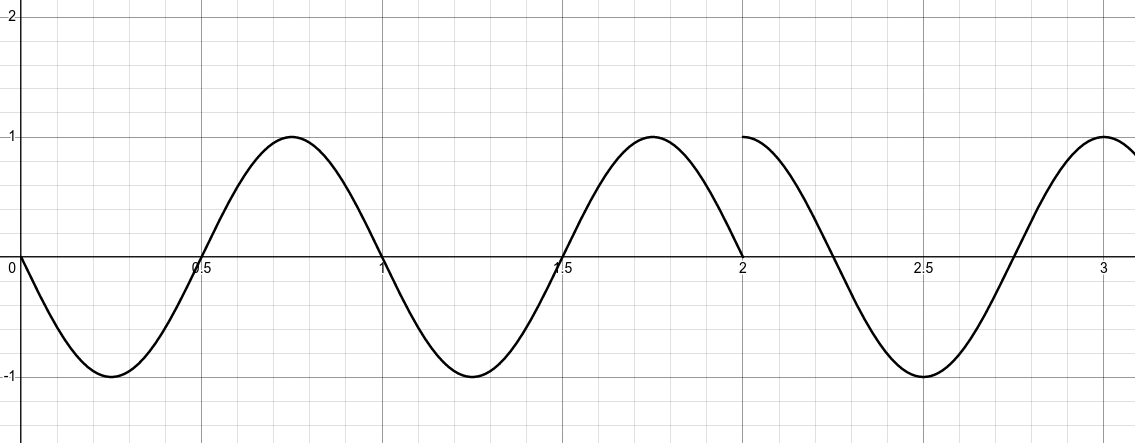
\includegraphics[width=.75\textwidth]{Figures/HW10-1f}
          \caption{Plot for $(B_1,B_2,B_3)=(1,1,0)$}
          \label{fig:6}
        \end{figure}

        \begin{figure}[H]
          \centering
          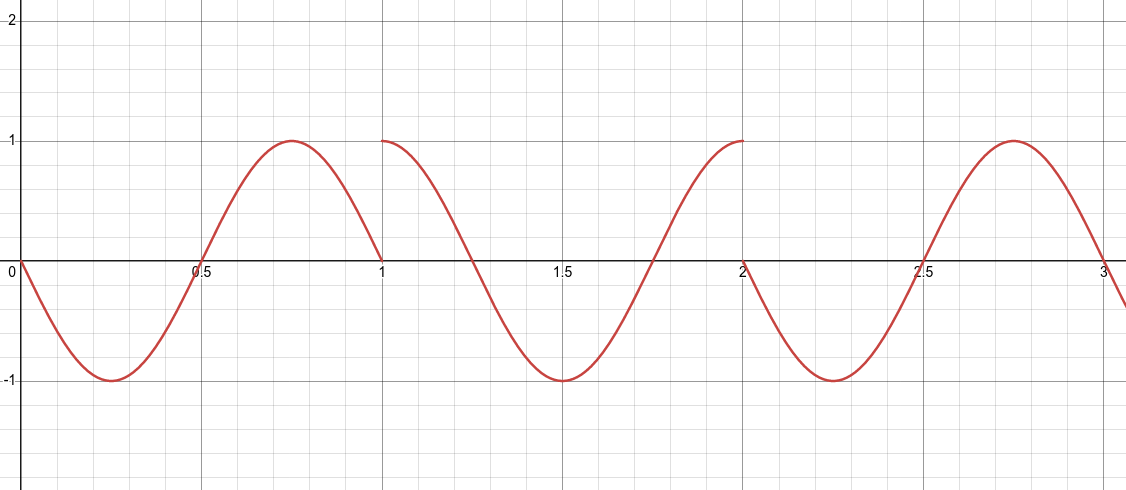
\includegraphics[width=.75\textwidth]{Figures/HW10-1g}
          \caption{Plot for $(B_1,B_2,B_3)=(1,0,1)$}
          \label{fig:7}
        \end{figure}

        \begin{figure}[H]
          \centering
          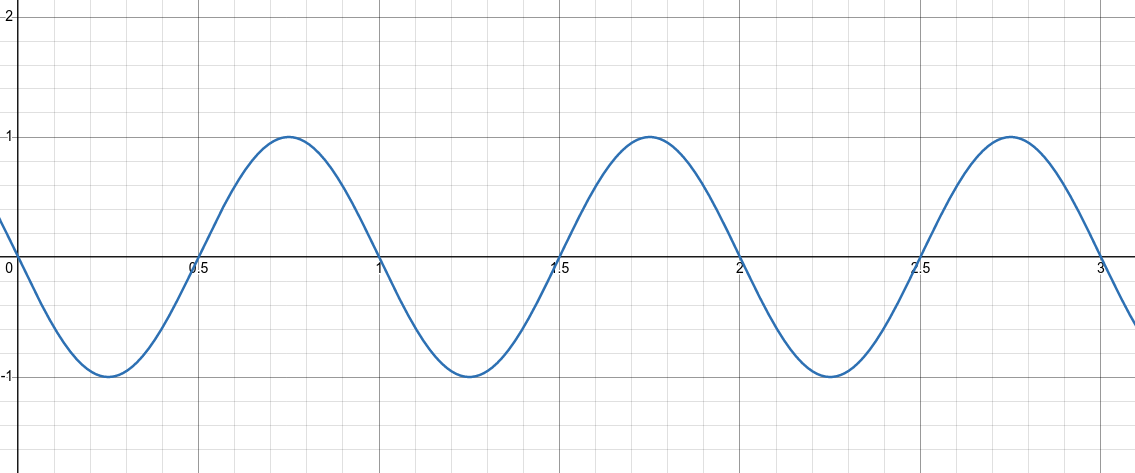
\includegraphics[width=.75\textwidth]{Figures/HW10-1h}
          \caption{Plot for $(B_1,B_2,B_3)=(1,1,1)$}
          \label{fig:8}
        \end{figure}

  \item

    \begin{enumerate}

      \item Taking $t\to100/3[\si{\micro\second}]$, we obtain:

        $$s_1=5\cos(10^4\pi (100/3)\cdot10^{-6})$$
        $$s_1=5\cos(\pi/3)$$
        $$s_1=2.5$$

        We can then find $Y_1(t)$ by tacking on the noise term to get:

        $$\boxed{Y_1(t)\to N(2.5,1)}$$

        Which means that this gives a normal distribution with a mean of 2.5 and standard deviation of 1.

      \item Similarly, we take $t\to100[\si{\micro\second}]$ to get:

        $$s_2=5\cos(10^4\pi 200\cdot10^{-6})$$
        $$s_2=5\cos(2\pi)$$
        $$s_2=5$$

        This gives us:

        $$\boxed{Y_2(t)\to N(5,1)}$$

        Or a normal distribution with mean 5 and standard deviation 1.

      \item Given that $s(t)$ is static, we know that the covariance depends solely on the noise. This gives us:

        $$\text{Cov}(Y_1,Y_2)=\text{Cov}(N_1,N_2)$$

        Since $N_1$ and $N_2$ are normal functions independent of each other, we find:

        $$\text{Cov}(Y_1,Y_2)=\text{Cov}(N_1,N_2)=0$$

        Which means that $Y_1$ and $Y_2$ are \underline{independent}

      \item Summing the two distributions and averaging their means and standard deviations, we find:

        $$E\left[ \frac{Y_1+Y_2}{2} \right]=\frac{1}{2}(5+2.5)$$
        $$E\left[ \frac{Y_1+Y_2}{2} \right]=3.75$$

        And then:

        $$\sigma_{(Y_1+Y_2)/2}=\left( \frac{1}{2} \right)^2(1+1)$$
        $$\sigma_{(Y_1+Y_2)/2}=.5$$

        Thus, we get:

        $$\boxed{\frac{Y_1(t)+Y_2(t)}{2}\to N(3.75,.5)}$$

        A normal distribution, with a mean of 3.75 and standard deviation of .5

    \end{enumerate}

    \setcounter{enumi}{3}

  \item

    \begin{enumerate}

      \item We know that the mean of $X(t)$ may be expressed as:

        $$\mu_X=E[X(t)]=E[A_o\cos(\omega_ot+\theta)]$$

        Given that this is over a uniform function from $-\pi$ to $\pi$, we find:

        $$\boxed{\mu_X=0}$$

        We proceed to find the autocorrelation function as:

        $$\mathcal{R}_{XX}(t,\tau)=E[X(t)X(t+\tau)]$$

        We expand to get:

        $$\mathcal{R}_{XX}(t,\tau)=E[A_o^2\cos(\omega_o t+\theta)\cos(\omega_o (t+\tau)+\theta)]$$

        Applying our cosine properties gives us:

        $$\mathcal{R}_{XX}(t,\tau)=E\left[\frac{A_o^2}{2}(\cos(\omega_o\tau)+\cos(2\omega_ot+\omega_o\tau))\right]$$

        This simplifies to:

        $$\boxed{\mathcal{R}_{XX}(t,\tau)=\frac{A_o^2}{2}\cos(\omega_o\tau)}$$

        As such, since the autocorrelation depends on the time difference, and the mean is constant, we may conclude that this \underline{is a wide-sense stationary process}

      \item We may write the mean as:

        $$\mu_y=E[V+X(t)]=E[V]+E[X(t)]$$

        This gives us:

        $$\boxed{\mu_y=\mu_V}$$

        We then write the autocorrelation function as:

        $$\mathcal{R}_{YY}(t,\tau)=E[Y(t)Y(t+\tau)]$$

        Expanding gives us:

        $$\mathcal{R}_{YY}(t,\tau)=E[(V+X(t))(V+X(t+\tau))]$$
        $$\mathcal{R}_{YY}(t,\tau)=E[V^2+VX(t+\tau)+VX(t)+X(t)X(t+\tau)]$$

        We then simplify to:

        $$\mathcal{R}_{YY}(t,\tau)=E[V^2+X(t)X(t+\tau)]$$
        $$\mathcal{R}_{YY}(t,\tau)=E[V^2]+E[X(t)X(t+\tau)]$$
        $$\boxed{\mathcal{R}_{YY}(t,\tau)=\sigma_V^2+\frac{A_o^2}{2}\cos(\omega_o\tau)}$$

        Since the mean is constant due to its independence from $\theta$, and the autocorrelation depends on the time difference, this \underline{is a wide-sense stationary function}

    \end{enumerate}

  \item

    \begin{enumerate}

      \item From the fact that $C(\tau)\neq C(-\tau)$, we may observe that this is \underline{not a valid} \underline{autocovariance function for a WSS random process}

      \item Although the given function is even, it does not satisfy the positive-definite requirement. That is, is does not follow:

        $$\sum_{i=1}^n\sum_{j=1}^n c_ic_j\mathcal{R}_x(\tau_i,\tau_j)\geq 0$$

        If we take $\tau_1=-1$ and $\tau_2=-2$, then we get:

        $$-c_1^2-2c_2^2$$

      We observe that this is less than zero, and, therefore, this is \underline{not a valid}\\ \underline{autocovariance function for a WSS random process}

      \item The function is even and non-negative for all of $\tau$, and it is positive definite. Therefore, we conclude that this is \underline{a valid autocovariance function for a WSS random process}. Note: we may verify that it is positive definite by showing that the sum would yield:

        $$c_ic_j\to \frac{1}{|\tau_1|}\frac{1}{|\tau_2|}$$

      Which must be positive.

      \item We may observe that the function is even, non-negative for all of $\tau$, and is positive definite. Therefore, we conclude that this \underline{is a valid autocovariance function for a} \underline{WSS random process}

    \end{enumerate}

  \item

    \begin{enumerate}

      \item We may observe that $X(t)$ \underline{is not periodic}, since the autocorrelation function does not contain a periodic term

      \item The function is not periodic, so we use the autocorrelation. We want to take $\tau\to \infty$; however, since $\tau$ is bounded, in this case, we take $\tau\to6$:

        $$E[X]=3-\frac{1}{2}(6)$$
        $$\boxed{E[X]=0}$$

      \item We may write the expected power as:

        $$E[X^2(t)]=\mathcal{R}_{XX}(0)$$

        This gives us:

        $$E[X^2(t)]=3-\frac{1}{2}(0)$$
        $$\boxed{E[X^2(t)]=3}$$

      \item We can express this using the value of the uniform distribution to get:

        $$P[X(t=1)>1]=\int_1^3\frac{1}{3-(-3)}\,dx$$
        $$P[X(t=1)>1]=\int_1^3\frac{1}{6}\,dx$$
        $$P[X(t=1)>1]=\frac{x}{6}\Big|_1^3$$
        $$P[X(t=1)>1]=\frac{3-1}{6}$$
        $$\boxed{P[X(t=1)>1]=\frac{1}{3}}$$

      \item We can break this up to write:

        $$E[(X(1)+X(2)+X(3))^2]=E[X^2(1)]+E[X^2(2)]+E{X^2(3)]+$$
        $$2E[X(1)X(2)]+2E[X(2)X(3)]+2E[X(1)X(3)]$$

        This is equivalent to:

        $$E[(X(1)+X(2)+X(3))^2]=3\mathcal{R}_{XX}(0)+4\mathcal{R}_{XX}(1)+2\mathcal{R}_{XX}(2)$$

        We evaluate to get:

        $$E[(X(1)+X(2)+X(3))^2]=3\left[ 3 \right]+4\left[ \frac{5}{2} \right]+2[2]$$
        $$\boxed{E[(X(1)+X(2)+X(3))^2]=23}$$

      \item Expanding, we get:

        $$E[Y]=2E[X]+3$$
        $$\boxed{E[Y]=3}$$

        We can then find:

        $$\mathcal{R}_{YY}(t)=E[(2X(t)+3)(2X(t+\tau)+3)]$$

        We expand this to get:

        $$\mathcal{R}_{YY}(t)=4E[X(t)2X(t+\tau)]+6E[X(t+\tau)]+6E[X(t)]+9$$
        $$\boxed{\mathcal{R}_{YY}(t)=4\mathcal{R}_{XX}(t)+9}$$

    \end{enumerate}

  \item

    \begin{enumerate}

      \item We may begin by computing the autocovariance as:

        $$C_{XX}(n,k)=\text{Cov}(X_n,X_k)$$

        But because all $X_n$ are i.i.d, we get:

        $$\boxed{C_{XX}(n,k)=\left\{\begin{array}{ll}\text{Var}(X_n), & n=k\\0, & n\neq k\end{array}}$$

        We then compute the autocorrelation as:

        $$R_{XX}(n,k)=E[X_nX_k]$$

        Because of independence, we write:

        $$R_{XX}(n,k)=E[X_n]E[X_k]$$

        Accordingly, we get:

        $$\boxed{R_{XX}(n,k)=\left\{\begin{array}{ll} p, & n=k\\ p^2, & n\neq k\end{array}}$$

      \item Since the distributions $X_n$ are i.i.d, we may obtain the probability as simply the sum of individual probabilites. Since the probability of each is the same, we get:

        $$\boxed{E[Y_n]=np}$$

        Similarly, we can sum the variances by writing:

        $$\text{Var}(Y_n)=n\text{Var}(X_n)$$
        $$\boxed{\text{Var}(Y_n)=np(1-p)}$$

      \item We may observe that each $X_n$ represents a Bernoulli trial. accordingly, since $Y_n$ is the sum of Bernoulli trials, it represents a Binomial distribution such that $\boxed{Y_n=\text{Binom}(n,p)}$

      \item We know that, to be a wide-sense stationary process, two conditions must be met:

        \begin{enumerate}

          \item $E[Y_n]$ is constant

          \item $\text{Cov}(Y_n,Y_k)$ is dependent solely on the difference $|n-k|$

        \end{enumerate}

        From (b), we see that $E[Y_n]=np$ is not constant, and, therefore, the process \underline{is not wide-sense stationary}.

      \item We begin by writing:

        $$C_{YY}(n,k)=\text{Cov}(Y_n,Y_k)$$

        This gives us:

        $$C_{YY}(n,k)=\sum_{i=1}^n\sum_{j=1}^k\text{Cov}(X_i,X_j)$$

        Given the independence of the distributions, we see that only diagonal terms remain, which means that the only non-zero covariances occur when:

        $$i=j\to \text{Cov}(X_i,X_j)=p(1-p)$$

        Therefore, we rewrite the above to get:

        $$C_{YY}(n,k)=\sum_{i=1}^{\text{min}(n,k)} p(1-p)$$

        As such, we finally get:

        $$\boxed{C_{YY}(n,k)=\text{min}(n,k)p(1-p)}$$

    \end{enumerate}

  \item

    \begin{enumerate}

      \item Given that $X$ and $Y$ are wide sense stationary processes, we may write:

        $$V(t)=2X(t)+Y(t)\to E[V]=2E[X]+E[Y]$$
        $$\mathcal{R}_V(t,\tau)=E[\bar{V}(t)V(t+\tau)]$$

        We expand this to get:

        $$\mathcal{R}_V(t,\tau)=E[(2X(t)+Y(t))(2X(t+\tau)+Y(t+\tau))]$$
        $$\mathcal{R}_V(t,\tau)=E[(2X(t)2X(t+\tau)+Y(t)Y(t+\tau))+2X(t)Y(t+\tau)+2Y(t)X(t+\tau)]$$

        And thus we conclude:

        $$\boxed{\mathcal{R}_V(t,\tau)\neq \mathcal{R}_X(t,\tau)+\mathcal{R}_Y(t,\tau)}$$

        Therefore, it is \underline{not wide sense stationary}

      \item Similar to the above, we write:

        $$E[W]=E[XY]$$

        Since $Y$ and $X$ are independent, we get:

        $$E[W]=E[X]E[Y]=\mu_X\mu_Y$$

        We then write:

        $$\mathcal{R}_W(t,\tau)=E[\bar{W}(t)W(t+\tau)]$$

        We expand:

        $$\mathcal{R}_W(t,\tau)=E[X(t)Y(t)X(t+\tau)Y(t+\tau)]$$

        Once again, because $X$ and $Y$ are independent, we get:

        $$\boxed{\mathcal{R}_W(t,\tau)=E[X(t)X(t+\tau)][EY(t)Y(t+\tau)]=\mathcal{R}_X(t,\tau)\mathcal{R}_Y(t,\tau)}$$

        And, therefore, $W$ \underline{is independent and wide sense stationary}

    \end{enumerate}

  \item We begin by writing the autocorrelation as:

    $$\mathcal{R}_{WW}(t,\tau)=E[W(t)W(t+\tau)]$$

    We expand to get:

    $$\mathcal{R}_{WW}(t,\tau)=E[(X\cos(10^8\pi t)+Y\sin(10^8\pi t))(X\cos(10^8\pi(t+\tau))+Y\sin(10^8\pi(t+\tau)))]$$

    Since $X$ and $Y$ are uncorrelated, we know that any expectation value involving both will cancel, so we simplify to:

    $$\mathcal{R}_{WW}(t,\tau)=E[X^2\cos(10^8\pi t)\cos(10^8\pi(t+\tau))+Y^2\sin(10^8\pi t)\sin(10^8\pi(t+\tau))]$$

    We use the identity that $\cos(x+y)=\cos(x)\cos(y)-\sin(x)\sin(y)$ to get:

    $$\mathcal{R}_{WW}(t,\tau)=E[X^2\cos(10^8\pi \tau)\cos(10^8\pi t)+Y^2\cos(10^8\pi\tau)\sin(10^8\pi t)]$$

    Since $X$ and $Y$ both have mean 0 and variance $\sigma^2$, we find that, as long as $t$ and $t+\tau$ are within the range of integration:

    $$\boxed{\mathcal{R}_{WW}(t,\tau)=\sigma^2\cos(10^8\pi (t-\tau))}$$

    Otherwise, it is zero.

    Accordingly, we observe that the process $W(t)$ \underline{is wide sense stationary}, since the mean is zero and the autocorrelation only depends on the time difference, $t-\tau$

    We can find the autocovariance as:

    $$C_{WW}(t,\tau)=R_{WW}(t,\tau)-E[W(t)]E[W(t+\tau)]$$

    Since we know the terms that go to zero, we find:

    $$C_{WW}(t,\tau)=R_{WW}(t,\tau)$$
    $$\boxed{C_{WW}(t,\tau)=\sigma^2\cos(10^8\pi (t-\tau))}$$

    We use the autocovariance to find:

    $$C_{WW}(0,.001)=\sigma^2\cos\left( -10^8\pi\cdot10^{-3} \right)$$
    $$C_{WW}(0,.001)=\sigma^2\cos\left( -10^5\pi \right)$$

    This simplifies to:

    $$\boxed{C_{WW}(0,.001)=\sigma^2}$$
    
    We can find the mean signal power by taking $\mathcal{R}_{WW}(0)$:

    $$E[W^2(t)]=\sigma^2\cos\left( 0 \right)$$
    $$\boxed{E[W^2(t)]=\sigma^2}$$

    Since the mean is zero, nothing is subtracted from the power, which gives us a variance of:

    $$\boxed{\text{Var}(W(t))=\sigma^2}$$

  \item We are given that the weather on each day is normally distributed with $E[W]=20[\si{\celsius}]$ and $\sigma=5[\si{\celsius}]$. Let us then express the two day-averaged distribution as:

    $$W_n=\frac{2X_n+X_{n-1}}{3}\quad\text{ and }\quad W_{n+1}=\frac{2X_{n+1}+X_n}{3}$$

    We find the Covariance between daily ``steps'' to get:

    $$\text{Cov}(W_n,W_{n+1})=\text{Cov}\left( \frac{2X_n+X_{n-1}}{3},\frac{2X_{n+1}+X_n}{3} \right)$$

    We can break this apart to get:

    $$\text{Cov}(W_n,W_{n+1})=\frac{1}{9}\left[2\text{Cov}\left( X_n,X_n \right)+4\text{Cov}\left( X_n,X_{n+1} \right)+2\text{Cov}\left( X_{n-1}. X_{n+1} \right)+\text{Cov}(X_{n-1},X_n)\right]$$
    $$\text{Cov}(W_n,W_{n+1})=\frac{1}{9}\left[2\text{Var}\left( X_n \right)\right]$$
    $$\boxed{\text{Cov}(W_n,W_{n+1})=\frac{50}{9}\left[ \si{\celsius\squared} \right]}$$

    Thus, since the covariance is not zero, the $W_n$ distributions are not independent, and, therefore it is \underline{not an i.i.d random sequence}.

    \setcounter{enumi}{11}

  \item

    \begin{enumerate}

      \item We may begin by constructing our distribution by using the formula for a Poisson distribution for each individual train line:

        $$P[n]=\frac{(\lambda T)e^{-\lambda T}}{n!}$$

        We combine the individual PMFs to get a general one for train arrivals as:

        $$\lambda= \lambda_R+\lambda_G+\lambda_B$$

        Entering the given information, we write:

        $$\lambda= .1+.05+.15$$
        $$\lambda= .3[\si{min^{-1}}]$$

        Accordingly, we find the quantity of trains in an hour as:

        $$\lambda T=60(.03)$$
        $$\lambda T=18[\si{trains/hour}]$$

        Applying this to our Poisson distribution formula, we find:

        $$\boxed{P_N[n]=\text{Poisson}(18)=\frac{(18)^ne^{-18}}{n!}}$$

      \item We want to find the conditional PMF, which we can do by constructing a binomial distribution

        $$P[R|N=10]=\left( \begin{matrix} 10\\ R \end{matrix} \right)\left( \frac{.1}{.3} \right)^R\left( 1-\frac{.1}{.3} \right)^{10-R} $$

        We simplify to find:

        $$\boxed{P[R|N=10]=\left( \begin{matrix} 10\\ R \end{matrix} \right)\left( \frac{1}{3} \right)^R\left( \frac{2}{3} \right)^{10-R}}$$

        As such, we see that this follows a binomial distrbution with $n=10$ and $p=1/3$

    \end{enumerate}

\end{enumerate}

\end{document}

